\section{Frontend: Visualizzazione Della Mappa}
\label{ch:frontend-advanced}

\subsection{Libreria scelta - Deck.gl}

In conclusione ho scelto di strutturare il progetto basandomi su \texttt{Deck.gl}, una libreria avanzata per la visualizzazione di dati geospaziali basata su WebGL. Un vantaggio significativo di Deck.gl è la capacità di lavorare direttamente con array di oggetti JavaScript (nel codice seguente, la variabile \texttt{data}), senza necessità di convertire i dati in formato GeoJSON. \cite{deckgl-heatmap} Il codice per la creazione di una heatmap risulta un buon esempio di tale compatibilità:

\begin{listing}[H]
\caption{Integrazione dati flat con Deck.gl}
\label{lst:deckgl_heatmap_layer} % Ho aggiunto un'etichetta per riferimento
\begin{minted}{javascript}
    const heatmapLayer = new deck.HeatmapLayer({
      id: 'heatmap',
      data: data,
      getPosition: d => [d.Longitude, d.Latitude],
      getWeight: d => d.Value
    });
\end{minted}
\end{listing}

Questa semplicità nella gestione dei dati lato frontend ha contribuito a mantenere l'interazione rapida e reattiva, anche in presenza di dataset di dimensioni non trascurabili. Inoltre, questo approccio sfrutta l'hardware GPU per il rendering di grandi quantità di dati e garantisce fluidità nell'interazione con mappe complesse. Questa performance è cruciale per garantire un'interazione reattiva quando si esplorano dataset di rumore subacqueo ad alta densità. \cite{deckgl-heatmap}

Oltre al rendering puro, Deck.gl offre:
\begin{itemize}
  \item \textbf{Layer specializzati} (tra cui \texttt{HeatmapLayer}) per visualizzazioni tematiche \cite{deckgl-docs}.
  \item \textbf{Supporto a WebGPU} futuro, che promette prestazioni ancora migliori su hardware compatibile \cite{deckgl-roadmap}.
  \item \textbf{Strumenti di monitoraggio} delle prestazioni e statistiche di disegno, utili in fase di sviluppo e ottimizzazione.
\end{itemize}

\subsection{Tema della UI}

Per conferire all'interfaccia un aspetto leggero e contemporaneo, è stato adottato lo stile \textbf{glassmorphism}, che simula superfici di vetro smerigliato sovrapposte \cite{glassmorphism-css}. La scelta di colorazioni pacate e dalla vividezza contenuta risalta le proprietà di queste superfici; si attua un compromesso che vede l'uso di minor dettagli a favore di una maggiore leggibilità dei testi. Colori, ombre, sfocature e contrasti diventano così metodi per veicolare informazioni e concetti. 

\begin{listing}[H]
\caption{Codice CSS per uno stile Glassmorphism}
\label{lst:css_glassmorphism} % Ho aggiunto un'etichetta per riferimento
\begin{minted}{css}
    .glass {
            background: rgba(255, 255, 255, 0.15);
            backdrop-filter: blur(12px);
            border: 1px solid rgba(255, 255, 255, 0.25);
            box-shadow: 0 8px 32px 0 rgba(31, 38, 135, 0.45);
    }
    
    .glass-dark {
            background: rgba(17, 25, 40, 0.9);
            backdrop-filter: blur(16px);
            border: 1px solid rgba(255, 255, 255, 0.15);
            box-shadow: 0 8px 32px 0 rgba(31, 38, 135, 0.5);
    }
\end{minted}
\end{listing}

A livello tecnico, questo design sfrutta filtri CSS moderni (`\texttt{backdrop-filter}`) insieme a trasparenze ed ombre morbide, per ottenere un effetto di profondità e stratificazione senza appesantire le prestazioni, in quanto si vuole dedicare la maggior parte delle risorse al rendering della mappa e dei punti del dataset.
Esempi tratti dall'implementazione effettiva sono consultabili in Figura \ref{fig:glass-overview}.

\begin{figure}[ht]
    \centering
    \begin{subfigure}{0.3\textwidth}
        \centering
        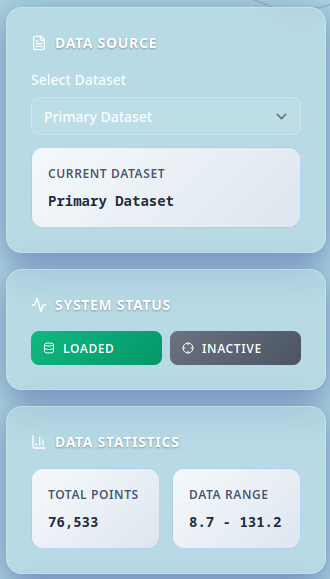
\includegraphics[width=\linewidth]{images/UI-glass-1.png}
        \caption{UI Glassmorphism 1}
        \label{fig:UI-glass-1}
    \end{subfigure}
    \qquad \qquad \qquad
    \begin{subfigure}{0.3\textwidth}
        \centering
        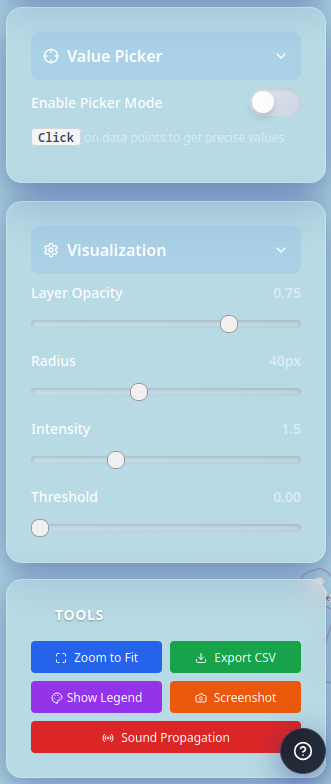
\includegraphics[width=\linewidth]{images/UI-glass-2.png}
        \caption{UI Glassmorphism 2}
        \label{fig:UI-glass-2}
    \end{subfigure}
    \caption{Esempi di Interfaccia Glassmorphism}
    \label{fig:glass-overview}
\end{figure}

\subsection{Design Responsivo}

Una delle priorità durante lo sviluppo è stata garantire la capacità del sito web di adattarsi in modo efficace al contenitore in cui viene visualizzato. La presenza congiunta di una mappa interattiva e di pannelli dotati di elementi di input eterogenei ha reso fondamentale la definizione di regole di \textit{layout} chiare e coerenti. 

Partizionare lo spazio della finestra in modo ordinato ha permesso di mantenere un'interfaccia leggibile e utilizzabile, indipendentemente dalle dimensioni dello schermo o dal livello di zoom applicato. In altre parole, l'obiettivo è stato quello di rendere l'interazione sempre fluida e accessibile, anche in condizioni di visualizzazione non ottimali.

Ho ritenuto quindi naturale l'uso di librerie in grado di portare a termine questo tipo di compito; l'intero layout è perciò basato su \textit{Tailwind CSS} ed arricchito da \textit{media queries} personalizzate, che consentono di identificare le dimensioni della finestra del browser e di conseguenza:
\begin{itemize}
  \item Ridimensionare automaticamente elementi dell'interfaccia quali griglie e container in base alla larghezza del viewport, ossia dello schermo del dispositivo utilizzato.
  \item Adattare la disposizione dei controlli per una fruizione ottimale su schermi piccoli \cite{tailwind-responsive}.
  \item Mantenere consistenza stilistica grazie alle \textit{utility class} predefinite \cite{tailwind-docs}.
\end{itemize}

Questo approccio assicura un'esperienza utente uniforme, indipendentemente dal dispositivo utilizzato.

\begin{figure}
    \centering
    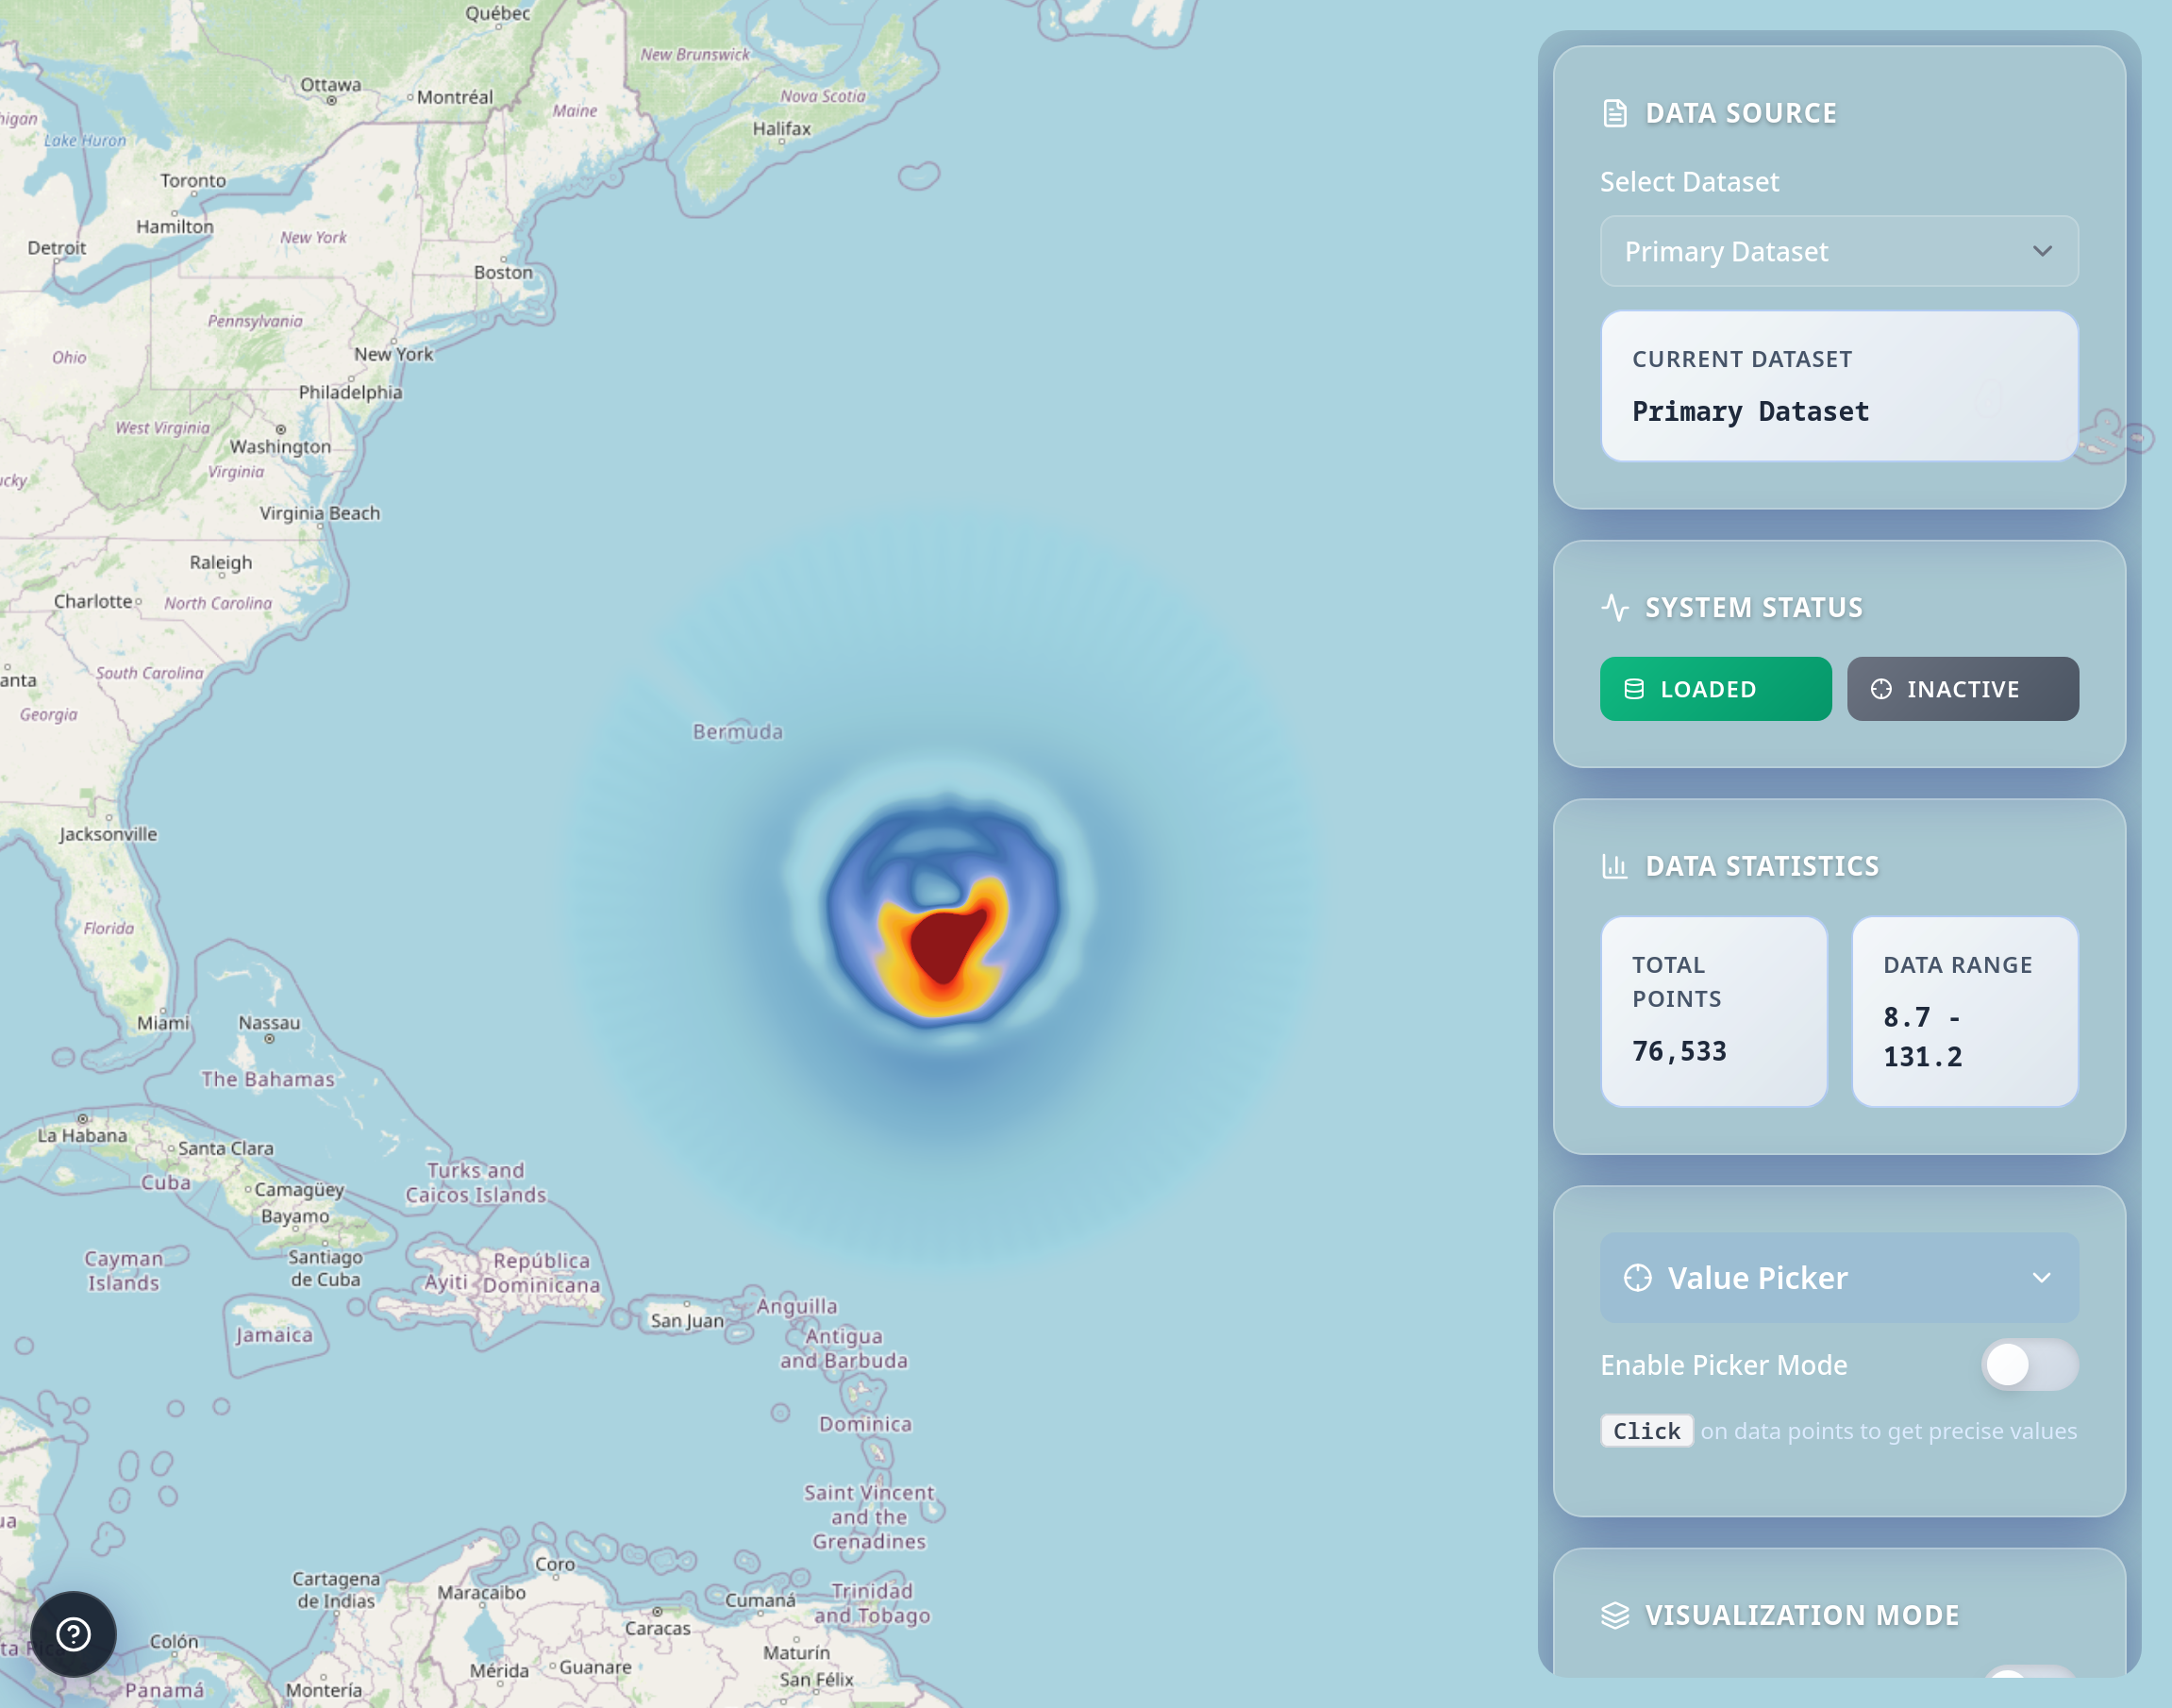
\includegraphics[width=0.86\linewidth]{images/whole-map-homepage.png}
    \caption{Interfaccia Web della Heatmap}
    \label{fig:heatmap-homepage}
\end{figure}

\subsection{Controlli Dinamici}

Per offrire un'esplorazione dei dati realmente interattiva, sono stati implementati \textit{widget} con pulsanti e slider che permettono di agire in tempo reale sulla visualizzazione (Figura \ref{fig:UI-glass-2}). Tali controlli sono in grado di variare le seguenti proprietà:

\begin{itemize}
  \item \textbf{Intensità Heatmap}: permette di regolare l'opacità della heatmap, rendendola trasparente a piacere; si utilizza per poter intravedere la mappa sottostante.
  \item \textbf{Raggio di Influenza}: Modifica la quantità di pixel su cui ogni punto influisce, variando la densità visiva delle aree.
  \item \textbf{Soglia di Visualizzazione}: Filtra i punti con valori inferiori a una soglia predefinita, eliminando il \say{rumore} dai dati.
  \item \textbf{Selezione Dataset}: Consente di passare istantaneamente tra più serie di dati, senza ricaricare l'intera pagina. (Figura \ref{fig:UI-glass-1})
\end{itemize}

Questi controlli sono collegati direttamente alle proprietà dei layer di Deck.gl, in modo da riflettere ogni modifica dell'utente senza ritardi. 
È possibile nascondere tutti i pannelli per una migliore visualizzazione della mappa sottostante tramite un apposito pulsante.

Inoltre il sistema integra un set di funzionalità progettate per ottimizzare l'interazione utente e l'analisi dei dati visualizzati. Queste caratteristiche mirano a fornire sia una visione d'insieme che un'analisi dettagliata, mantenendo al contempo un'interfaccia utente intuitiva.

\subsubsection*{Value Picker} Questa funzionalità trasforma la Heatmap in uno strumento di interrogazione precisa. Attivabile tramite un interruttore \say{Enable picker mode}, essa consente all'utente di selezionare punti specifici sulla mappa; passando con il cursore su qualsiasi punto apparirà un riquadro in cui sono indicate le coordinate geografiche (Latitudine/Longitudine) e il valore numerico esatto del punto selezionato. Tale precisione è cruciale per l'analisi puntuale dei dati. Cliccando su un punto della mappa si potranno copiare tali valori.

\subsubsection*{Statistiche Dati}
Questa sezione offre una panoramica sintetica e immediata del dataset in uso. L'elemento \say{Total Points}, che indica il numero totale di datapoint visualizzati, fornisce una stima della densità dei dati, mentre \say{Data Range} specifica l'intervallo dei valori presenti nel dataset (minimo e massimo), fornendo informazioni sulla scala dei fenomeni rappresentati.

\begin{figure}
    \centering
    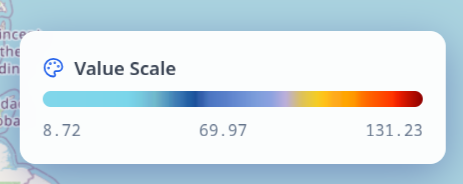
\includegraphics[width=0.5\linewidth]{images/legenda.png}
    \caption{Legenda}
    \label{fig:legenda}
\end{figure}

\subsubsection*{Legenda Colori}
Elemento interpretativo fondamentale, la Legenda Colori (in Figura \ref{fig:legenda}) facilita la comprensione del mapping tra colori e valori numerici. Caratterizzata da un \say{Gradiente dinamico}, la scala dei colori si adatta automaticamente al \say{Range valori} del dataset corrente, massimizzando la differenziazione visiva. Vi è un pulsante che permette all'utente di mostrare o nascondere la legenda per ottimizzare lo spazio o la pulizia visiva, mentre le etichette numeriche che si trovano sotto la barra colorata forniscono riferimenti chiari ai valori minimo e massimo del gradiente, essenziali per una corretta interpretazione quantitativa della Heatmap.

\subsection{Simulazione Propagazione}

Il sistema adotta un modello di propagazione acustica fondato sui principi fisici dell'acustica subacquea. La velocità di propagazione è fissata a 1481 m/s, un valore di riferimento comunemente accettato per la velocità del suono in acqua marina, corrispondente a condizioni standard di temperatura e salinità negli ambienti oceanici.

La propagazione viene modellata attraverso un'espansione concentrica, che considera sia la geometria dello spazio che le caratteristiche fisiche del mezzo. Il fronte d'onda si diffonde radialmente a partire dalla sorgente, mentre l'intensità del segnale è modulata in funzione della distanza, seguendo i principi dell'attenuazione geometrica e tenendo conto delle proprietà dissipative del mezzo, desunte dai valori di intensità contenuti nei dataset.

\begin{figure}[htbp]
    \centering
    % Primo frame
    \begin{subfigure}{0.32\textwidth}
        \centering
        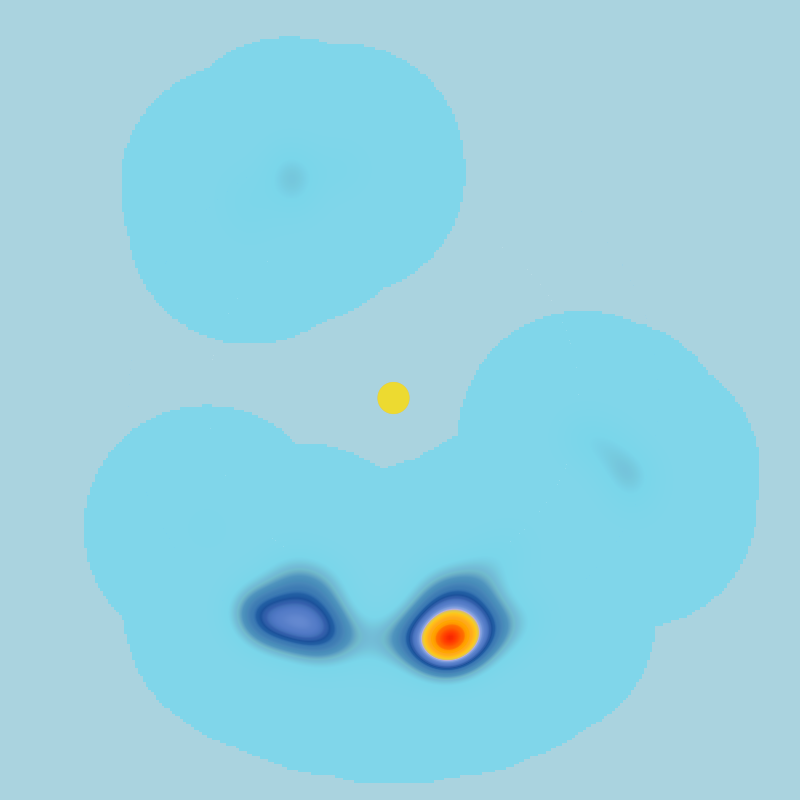
\includegraphics[width=\linewidth]{images/propagation-1.png}
        \caption{Momento iniziale} % Didascalia specifica
        \label{fig:propagation-frame-1} % Etichetta specifica
    \end{subfigure}
    \hfill % Spazio flessibile
    % Secondo frame
    \begin{subfigure}{0.32\textwidth}
        \centering
        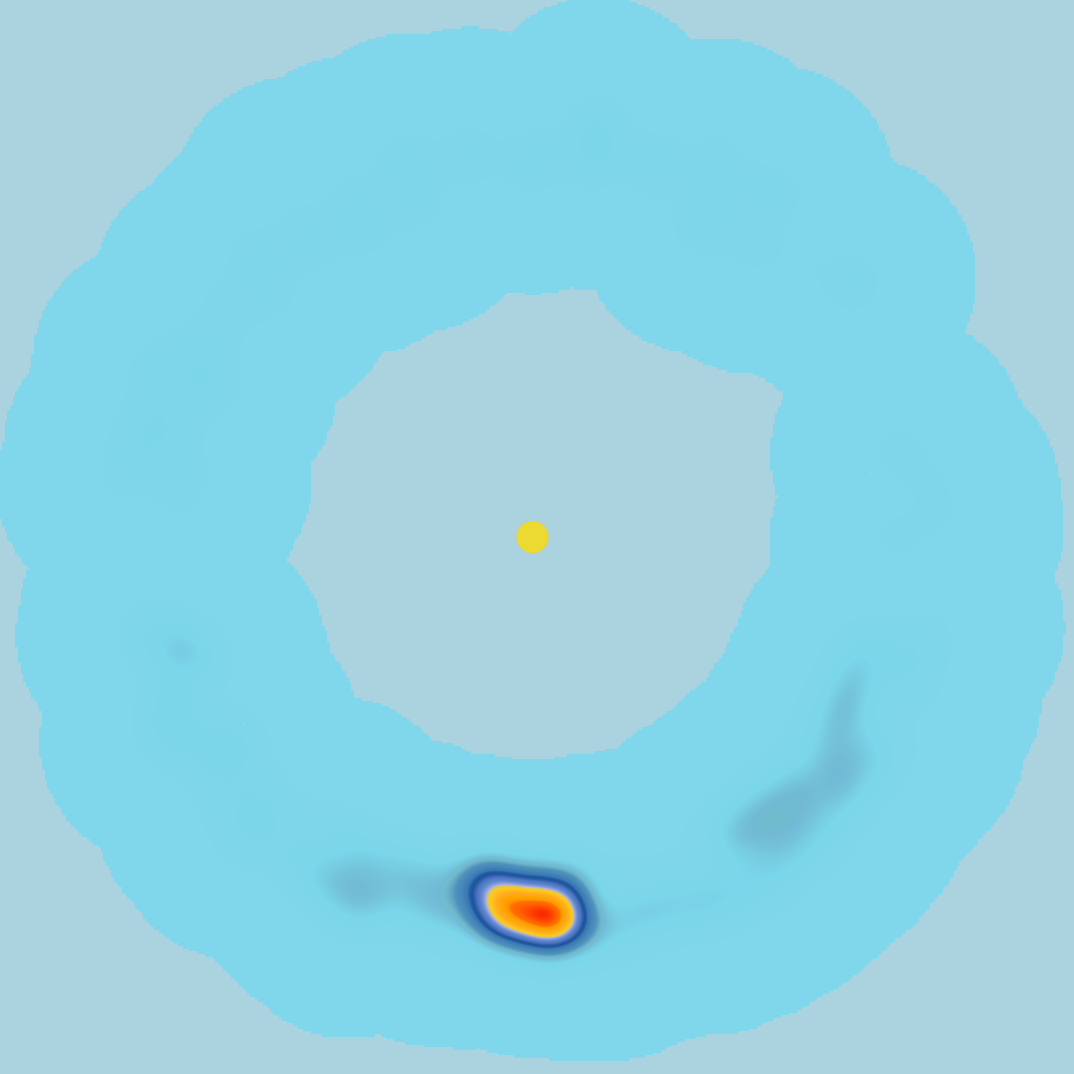
\includegraphics[width=\linewidth]{images/propagation-2.png}
        \caption{Propagazione intermedia} % Didascalia specifica
        \label{fig:propagation-frame-2} % Etichetta specifica
    \end{subfigure}
    \hfill % Spazio flessibile
    % Terzo frame
    \begin{subfigure}{0.32\textwidth}
        \centering
        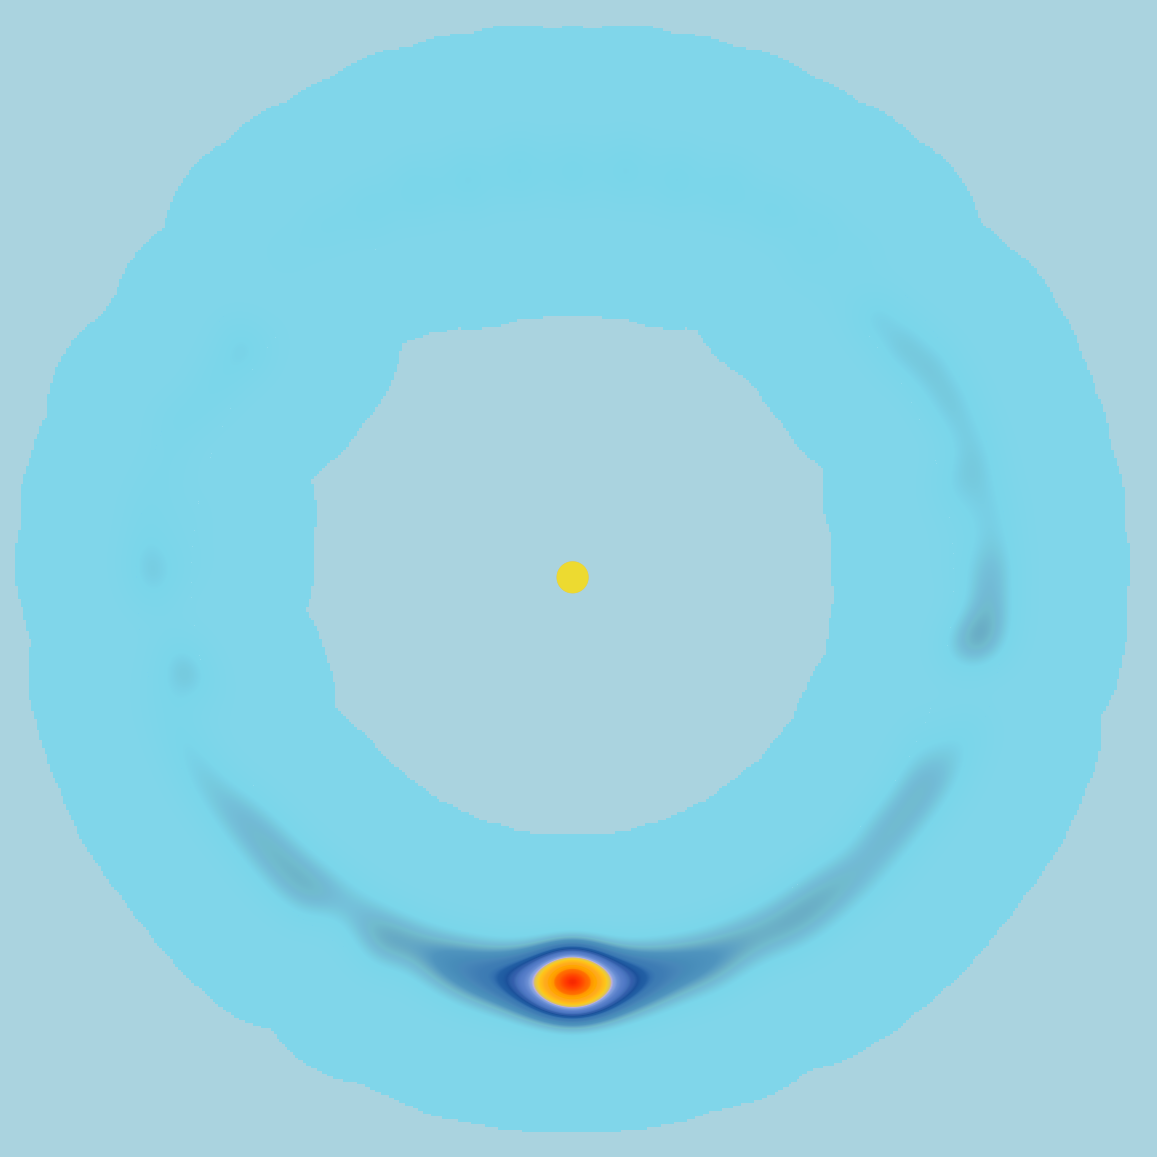
\includegraphics[width=\linewidth]{images/propagation-3.png}
        \caption{Propagazione avanzata} % Didascalia specifica
        \label{fig:propagation-frame-3} % Etichetta specifica
    \end{subfigure}
    
    \caption{Sequenza di frame illustranti l'evoluzione di un'animazione di propagazione.} % Didascalia generale
    \label{fig:propagation-animation-overview} % Etichetta generale
\end{figure}